\documentclass[12pt,a4paper,UTF8]{article}
\usepackage{ctex} % Chinese support
\usepackage{graphicx} % Insert images
\usepackage{subfigure}
\usepackage{float}
\usepackage{listings} % Print source code
\usepackage{color} % Color support
\usepackage{booktabs} % Professional table support
\usepackage{pdflscape} % Landscape pages support in PDF
\usepackage{hyperref} % Hypertext links support for cross-referencing
\usepackage{amsmath,mathtools}
\usepackage{ulem} % strikethrough

% Customize hyperref format (it's set to no special format here)
\hypersetup{hidelinks}

% Declare directories to search for graphics files for graphicx
\graphicspath{{figures/}}

% Define source code style for listings
\lstdefinestyle{verilog-style}{
	language=Verilog,
	basicstyle=\ttfamily\footnotesize,
	keywordstyle=\bfseries\color[rgb]{0, 0, 1},
	identifierstyle=\color[rgb]{0.5, 0.3, 0.1},
	stringstyle=\color[rgb]{0.6, 0.1, 0.1},
	commentstyle=\itshape\color[rgb]{0.05, 0.5, 0.05},
	backgroundcolor=\color[gray]{0.95},
	numbers=left,
	numbersep=5pt,
	numberstyle=\color[gray]{0.6},
	breaklines=true
}

\newcommand{\reporttitle}[2]{
  \LARGE\textsf{#1}\quad\underline{\makebox[12em]{#2}}
}

\newcommand{\reportinfo}[2]{
  \large\makebox[4em]{\textsf{#1}}\quad\underline{\makebox[18em]{#2}}
}

\begin{document}
\begin{titlepage}
  \centering
  \vspace*{\fill}
  {\Huge\textsf{数字电路与数字系统实验}} \\ [100pt]
  \reportinfo{实验名称}{exp08 状态机及键盘输入} \\ [10pt]
  \reportinfo{院系}{计算机科学与技术系} \\ [10pt]
  \reportinfo{学生姓名}{} \\ [10pt]
  \reportinfo{学号}{} \\ [10pt]
  \reportinfo{班级}{数字电路与数字系统实验1班} \\ [10pt]
  \reportinfo{邮箱}{} \\ [10pt]
  \reportinfo{实验时间}{2020 年 10 月 19 日} \\ [10pt]
  \vspace*{\fill}
\end{titlepage}
\tableofcontents
\newpage

\section{实验目的}
\begin{itemize}
  \item 复习有关状态机的知识
  \item 学习在Verilog编程中运用状态机的原理
  \item 了解状态机的编码方式
  \item 设计PS/2键盘控制器
  \item 练习Verilog多模块编程以及
        时钟、存储器、状态机的综合运用
\end{itemize}

\section{实验原理}
\begin{itemize}
  \item 有限状态机的原理
  \item PS/2接口的工作时序原理
  \item 键盘扫描码---键盘键值---键盘ASCII码的转换表格
  \item Verilog实现FIFO队列对读取键盘数据的缓冲
\end{itemize}

\section{实验环境/器材}
\begin{itemize}
  \item Quartus编辑器和DE10-Standard开发平台
  \item FPGA开发板
  \item 带有PS/2接口的键盘
\end{itemize}

\section{程序思路和代码}
\subsection{模块结构}
\label{bsec:struct}
因为要实现一个控制键盘的Verilog程序,所以我们首先封装
一个控制键盘的接口模块\mbox{out\_kbd},在顶层模块中直接调用
该模块即可。在该模块\linebreak[4]
\mbox{out\_kbd}中,我们调用题目中给出的\mbox{ps2\_keyboard}
模块,得到扫描码data以及ready等数据和信号。
根据这些信号我们在\mbox{out\_kbd}模块中编写一个always\linebreak[4]
块,处理这些数据然后得到有效的扫描码\mbox{eff\_data}
(不读取断码F0)、按键次数keystrokes、
读指针前移信号\mbox{nextdata\_n}、
以及输出大小写信号\mbox{kbd\_type}。将\mbox{kbd\_type}和
\mbox{eff\_data}传入\mbox{roms\_ascii}模块,得到对应数据的
ASCII码\mbox{ascii\_vec}。最后用模块\mbox{seg\_7\_out},
把要输出的十六进制数据转换成七段数码管格式的数据,然后输出。

\begin{figure}[H]
  \centering
  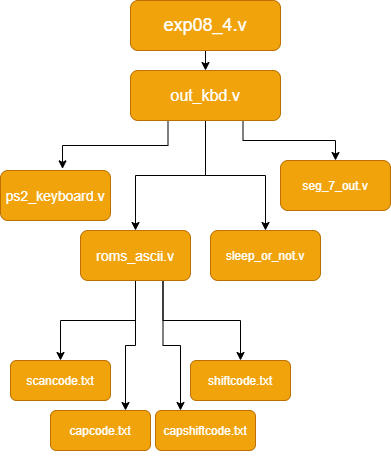
\includegraphics[width=0.8\textwidth]{code_struct.PNG}
  \caption{模块结构}
  \label{struct}
\end{figure}

\subsection{具体实现}
\mbox{ps2\_keyboard}的实现原理在题目中已经描述得很清楚了,
这里就略过不进行解释了。下面主要解释一下其他几个模块。

\subsubsection{输出按键的ASCII码}
\label{bbsec:ascii}
区分大小写和两个按键有关:CapsLock和Shift。键盘字母默认输出为小写。
双字符键默认输出下档字符。按一次CapsLock后,启动大写锁定状态,
所有字母输出转成大写,再按一次CapsLock后恢复小写状态。小写状态且
Shift键被按住时,双字符键输出上档字符,所有字母都输出为大写字母。
大写锁定状态时且Shift键被按住时,双字符键同样输出上档字符,但所有字母
输出为小写。

对于这四种情况,分别构建四个存储器存储每个扫描码对应的ASCII码。用case
语句选择当前情况对应的存储器输出ASCII码,封装成模块\mbox{roms\_ascii}\linebreak[4]
如下:
\begin{lstlisting}[style=verilog-style]
module roms_ascii(kbd_type, addr, dout_vec);
   input [1:0] kbd_type; // normal, cap, shift, capshift 
   input [7:0] addr;
   output reg [7:0] dout_vec;
   
   reg [7:0] normcode[255:0];
   reg [7:0] capcode[255:0];
   reg [7:0] shiftcode[255:0];
   reg [7:0] capshiftcode[255:0];
   initial begin
      dout_vec = 8'b0;
      $readmemh("D:/source/quartus/exp08_4/scancode.txt", normcode, 0, 255);
      $readmemh("D:/source/quartus/exp08_4/capcode.txt", capcode, 0, 255);
      $readmemh("D:/source/quartus/exp08_4/shiftcode.txt", shiftcode, 0, 255);
      $readmemh("D:/source/quartus/exp08_4/capshiftcode.txt", capshiftcode, 0, 255);
   end
      
   always @ (*) begin
      case (kbd_type)
         2'd0: dout_vec = normcode[addr];
         2'd1: dout_vec = capcode[addr];
         2'd2: dout_vec = shiftcode[addr];
         2'd3: dout_vec = capshiftcode[addr];
         default: dout_vec = 8'bz;
      endcase
   end
endmodule
\end{lstlisting}

这里解释一下为什么不用.mif文件而是用.txt文件初始化存储器。
因为写测试文件进行仿真运行时,如果程序中有.mif文件的话,
会出现一些奇奇怪怪的问题,比如初始化失败之类。为了避免这些问题,
我直接通过绝对地址引用.txt文件来初始化存储器。

\subsubsection{松开按键后熄灭输出}
要实现按键松开时,七段数码管低四位(ASCII码和键码)全灭,
我们需要知道松开时键盘向程序发送了什么样的数据。根据实验题目中
所述,PS/2接口数据传送顺序为:起始位(1'b0)+ 八位数据位
(由低到高)+ 奇校验位 + 停止位(1'b1)。我们推测知松开按键后,
键盘向程序发送的数据帧一直是``1''。所以我们可以这样实现熄灭输出功能:
当键盘向程序发送的数据帧连续一段时间都是``1''后,输出熄灭,直到
程序接收到数据帧``0'',再重新恢复输出。
\begin{lstlisting}[style=verilog-style]
module sleep_or_not(clk, ps_data, tosleep);
   input clk, ps_data;
   output reg tosleep;
   
   parameter [31:0] lim = 100000000; // default 10000000
   integer cnt;

   initial begin
      cnt = 0;
      tosleep = 0;
   end
   
   always @ (posedge clk) begin
      if (ps_data == 0) begin
         cnt <= 0;
         tosleep <= 0;
      end else begin
         if (tosleep == 1 || cnt == lim) begin
            cnt <= lim;
            tosleep <= 1;
         end else begin
            cnt <= cnt + 1;
            tosleep <= 0;
         end
      end
   end 
endmodule 
\end{lstlisting}

\subsubsection{扫描码的处理}
处理扫描码主要是在\mbox{out\_kbd}模块中,该模块处理完扫描码后
会通过调用\mbox{roms\_ascii}、\mbox{seg\_7\_out}等模块进行输出。
调用模块的功能详见前文\ref*{bsec:struct}节,本节主要描述对特殊的
扫描码的处理以及与之相关的状态赋值。

首先是按键次数的统计。我先尝试在按下键时计数,用一个存储器记录每个键
是否被按下的状态。按下时存储器对应元素置1,松开时置0,上升沿时按键
次数加一。但是实际操作时,却遇到了各种奇怪的按键抖动而重复计数。于是
我改成了在松开按键时计数。代码逻辑如下:
\begin{itemize}
  \item 当扫描码刚刚读到F0时,按键次数加一。在读到另一个扫描码之前\linebreak[4]
        \mbox{has\_counted}信号一直置1,不再重复计数。
  \item 当扫描码是F0时pressed一直置0,其他情况置1。
        在其上升沿时,当前的data就是当前松开的按键。如果
        当前data是大写锁定键的键码,那么就取反大写锁定状态
        (\mbox{kbd\_type[0]})。
  \item 剩下部分是判断Shift的状态。当data是Shift的键码时,
        Shift的状态(\mbox{kbd\_type[1]})置为1;当读到F0之后的
        data是Shift的键码时,Shift的状态置为0,同时\mbox{shift\_off}
        置为1,经过一段固定的时间之后再置为0。当\mbox{shift\_off}为1时,
        Shift的状态一直置为0。此信号的目的是取分Shift的断码和通码,
        在遇到Shift的断码时不把Shift的状态置为1。
\end{itemize}
\begin{lstlisting}[style=verilog-style]
initial begin
  nextdata_n = 1;
  shift_off = 0;
  pressed = 1;
  has_counted = 0;
  kbd_type = 2'b0;
  eff_data = 8'b0;
  keystrokes = 0;
  cnt_shift = 0;
end

always @ (posedge clk) begin
  if (clrn == 0) begin
     nextdata_n <= 1;
     shift_off <= 0;
     pressed <= 1;
     has_counted <= 0;
     kbd_type <= 2'b0;
     eff_data <= 8'b0;
     keystrokes <= 0;
     cnt_shift <= 0;
  end else begin
     if (ready) begin 
        if (data == 8'hF0) begin // don't read F0
           pressed <= 0;
           if (has_counted == 0) begin
              keystrokes <= keystrokes + 1;
              has_counted <= 1;
           end 
        end else begin
           has_counted <= 0;
           if (pressed == 0) begin
              pressed <= 1;
              if (data == 8'h58) kbd_type[0] <= ~kbd_type[0]; // Caps
              if (data == 8'h12 || data == 8'h59) begin // shift off
                 kbd_type[1] <= 0;
                 shift_off <= 1;
              end
           end else begin
              eff_data <= data;
              if ((data == 8'h12 || data == 8'h59) && shift_off == 0) begin
                 kbd_type[1] <= 1; // shift on
              end
           end
        end
        nextdata_n <= 0; 
     end else nextdata_n <= 1;
  
     // delay for next shift
     if (shift_off) begin
        if (cnt_shift == 10000000) begin
           cnt_shift <= 0;
           shift_off <= 0;
        end else begin
           cnt_shift <= cnt_shift + 1;
           shift_off <= 1;
        end
     end 
     
  end
end
\end{lstlisting}

\subsubsection{FPGA引脚分配}
本次实验主要通过键盘操作。比起前几个实验,FPGA用到的引脚少了很多。
除了FPGA提供的时钟信号,我把\mbox{KEY[0]}作为清零按钮,
\mbox{LEDR[0]}作为大写锁定信号,\mbox{LEDR[1]}作为Shift信号。
此外,我们只要根据题目要求,分配一下6个七段数码管就完成了。

\begin{lstlisting}[style=verilog-style]
\end{lstlisting}

\section{测试方法}
测试文件参照实验题目中给出的两个仿真模块即可。我们先用\mbox{test bench}\linebreak[4]
生成一个默认的测试文件,然后按照实验题目中的\mbox{keyboard\_sim}
模块修改。即除了保留主模块调用和参数声明之外,其他全部复制粘贴
\mbox{keyboard\_sim}模块的代码(相应参数如果名称不同则需要修改)。
接下来我们手动新建一个\mbox{ps2\_keyboard\_model.vt}文件,
把\mbox{ps2\_keyboard\_model}模块全文复制粘贴到该文件中,
然后把这个文件放到modelsim文件夹中。最后打开:\\
\fbox{Assignments$\rightarrow$Settings$\rightarrow$Simulation$\rightarrow$Compile test bench}\\
把刚刚的两个vt文件都添加进来,添加完成后如下图:
\begin{figure}[H]
  \centering
  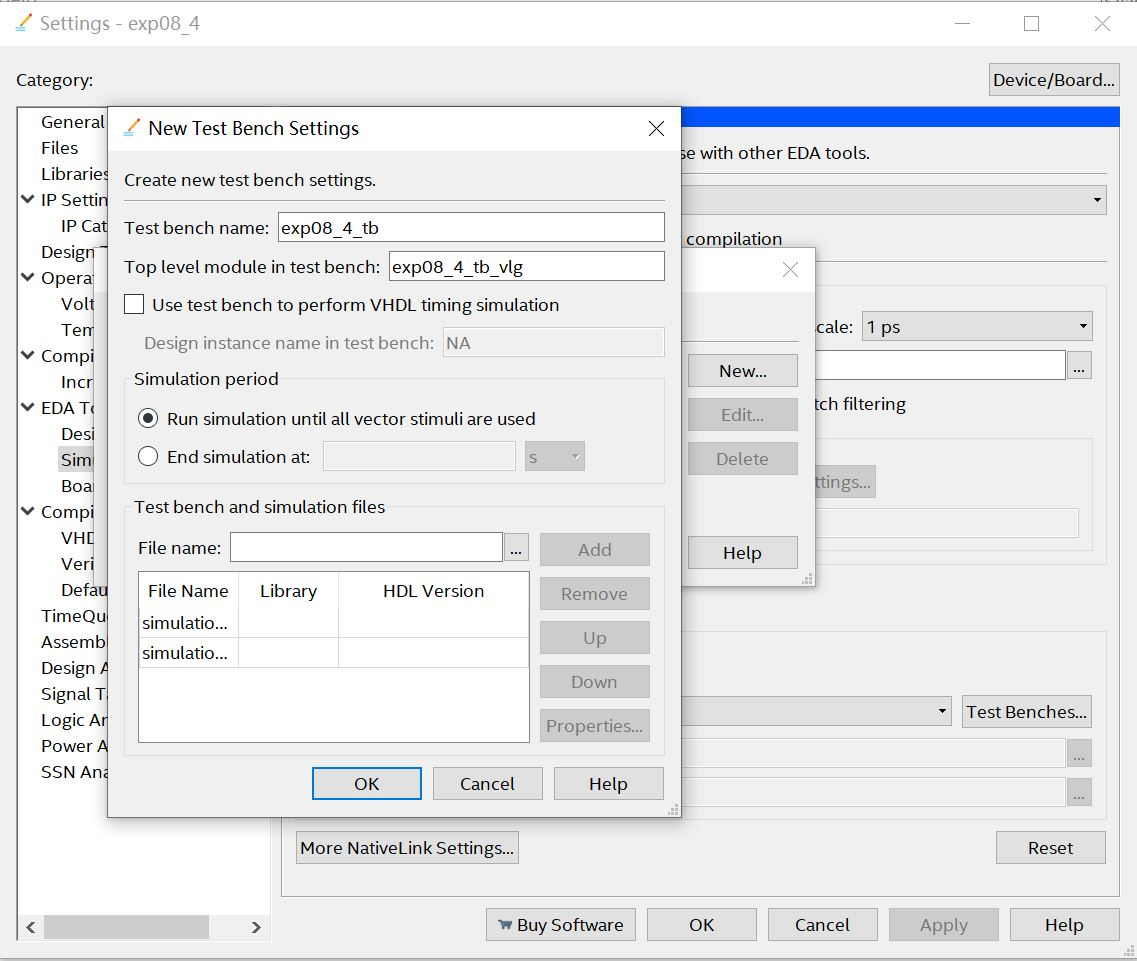
\includegraphics[width=1\textwidth]{sim_settings.JPG}
  \caption{添加测试文件}
  \label{set}
\end{figure}

运行结果如下:
\begin{figure}[H]
  \centering
  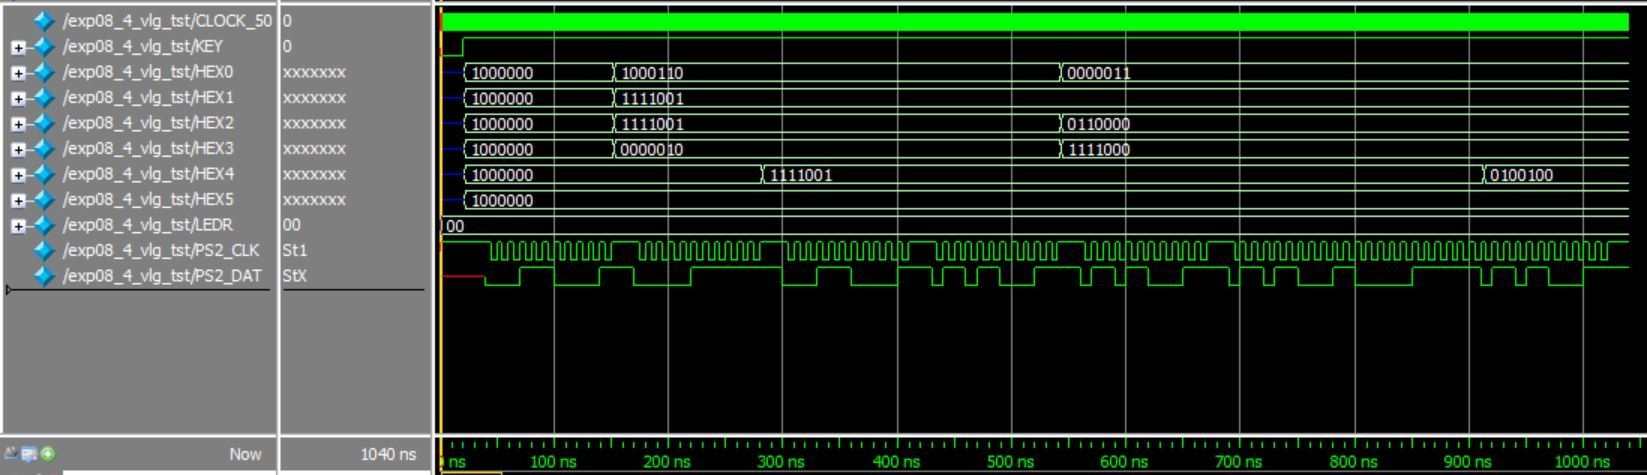
\includegraphics[width=1\textwidth]{sim.JPG}
  \caption{仿真运行结果}
  \label{sim}
\end{figure}

\section{实验结果}
在FPGA开发板上运行如下:
\begin{figure}[H]
  \centering
  \subfigure[FPGA initial]{
    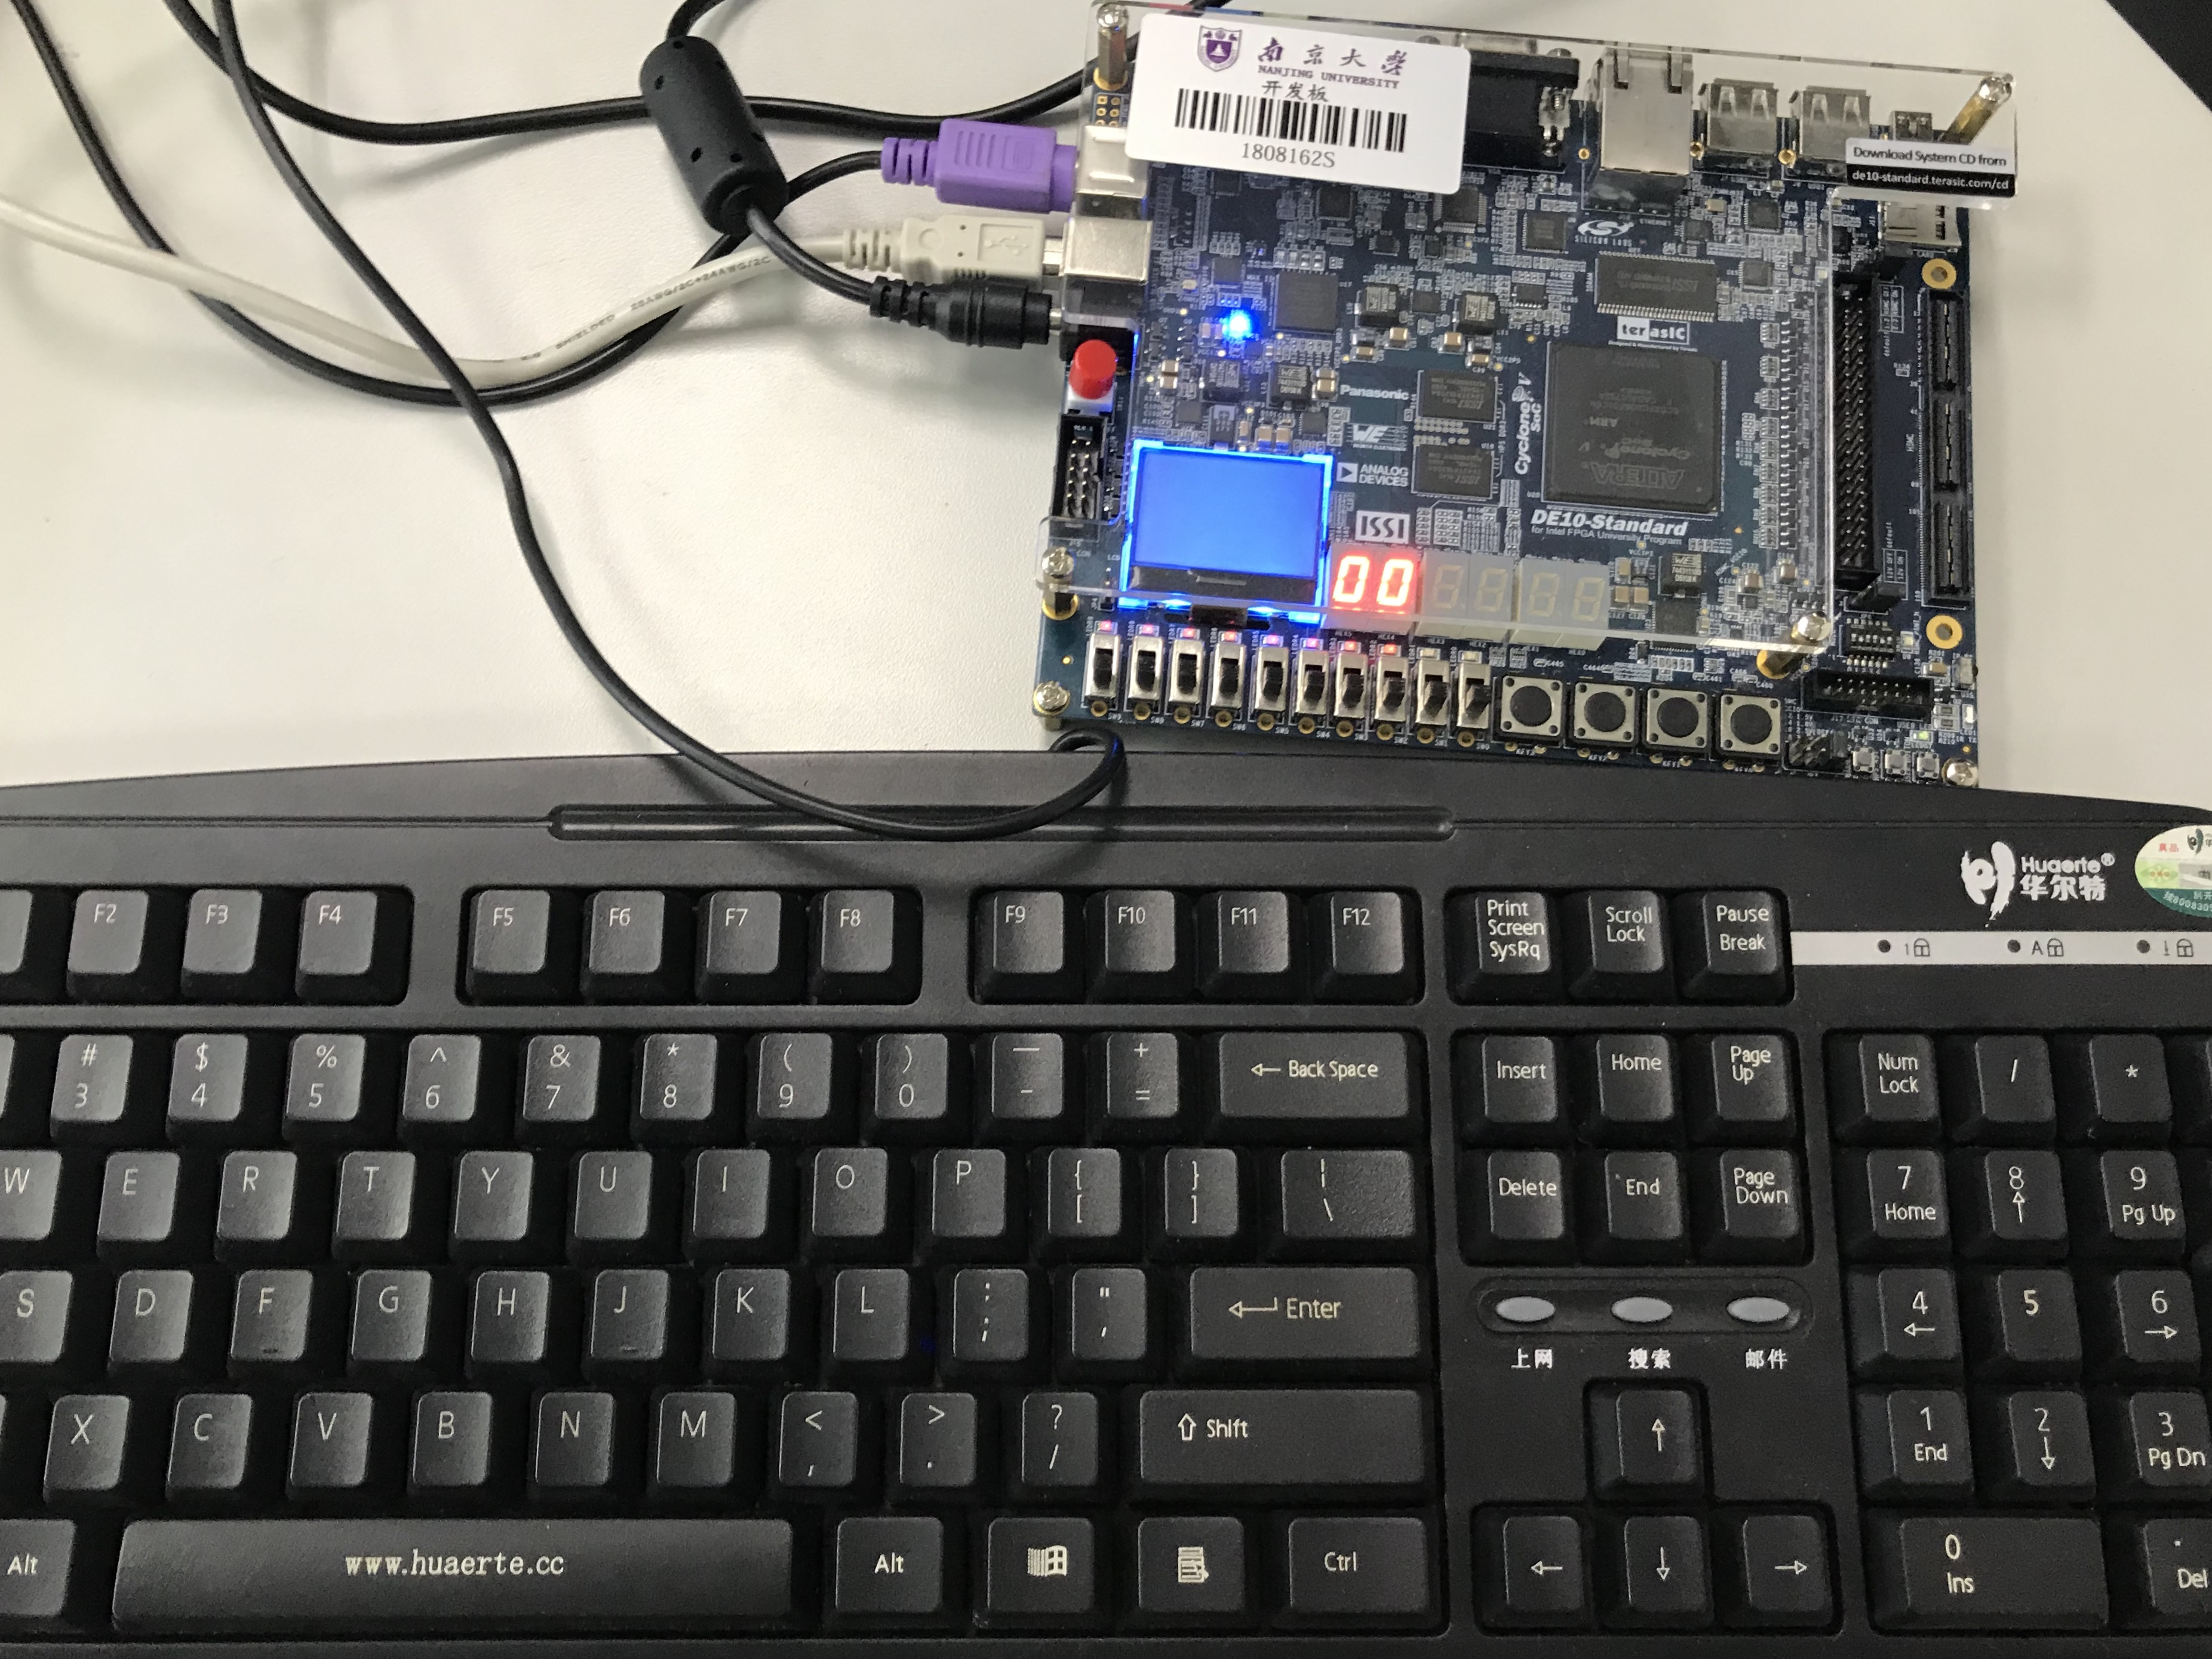
\includegraphics[width=0.45\textwidth]{fpga_init.JPG}
  }
  \subfigure[FPGA normal]{
    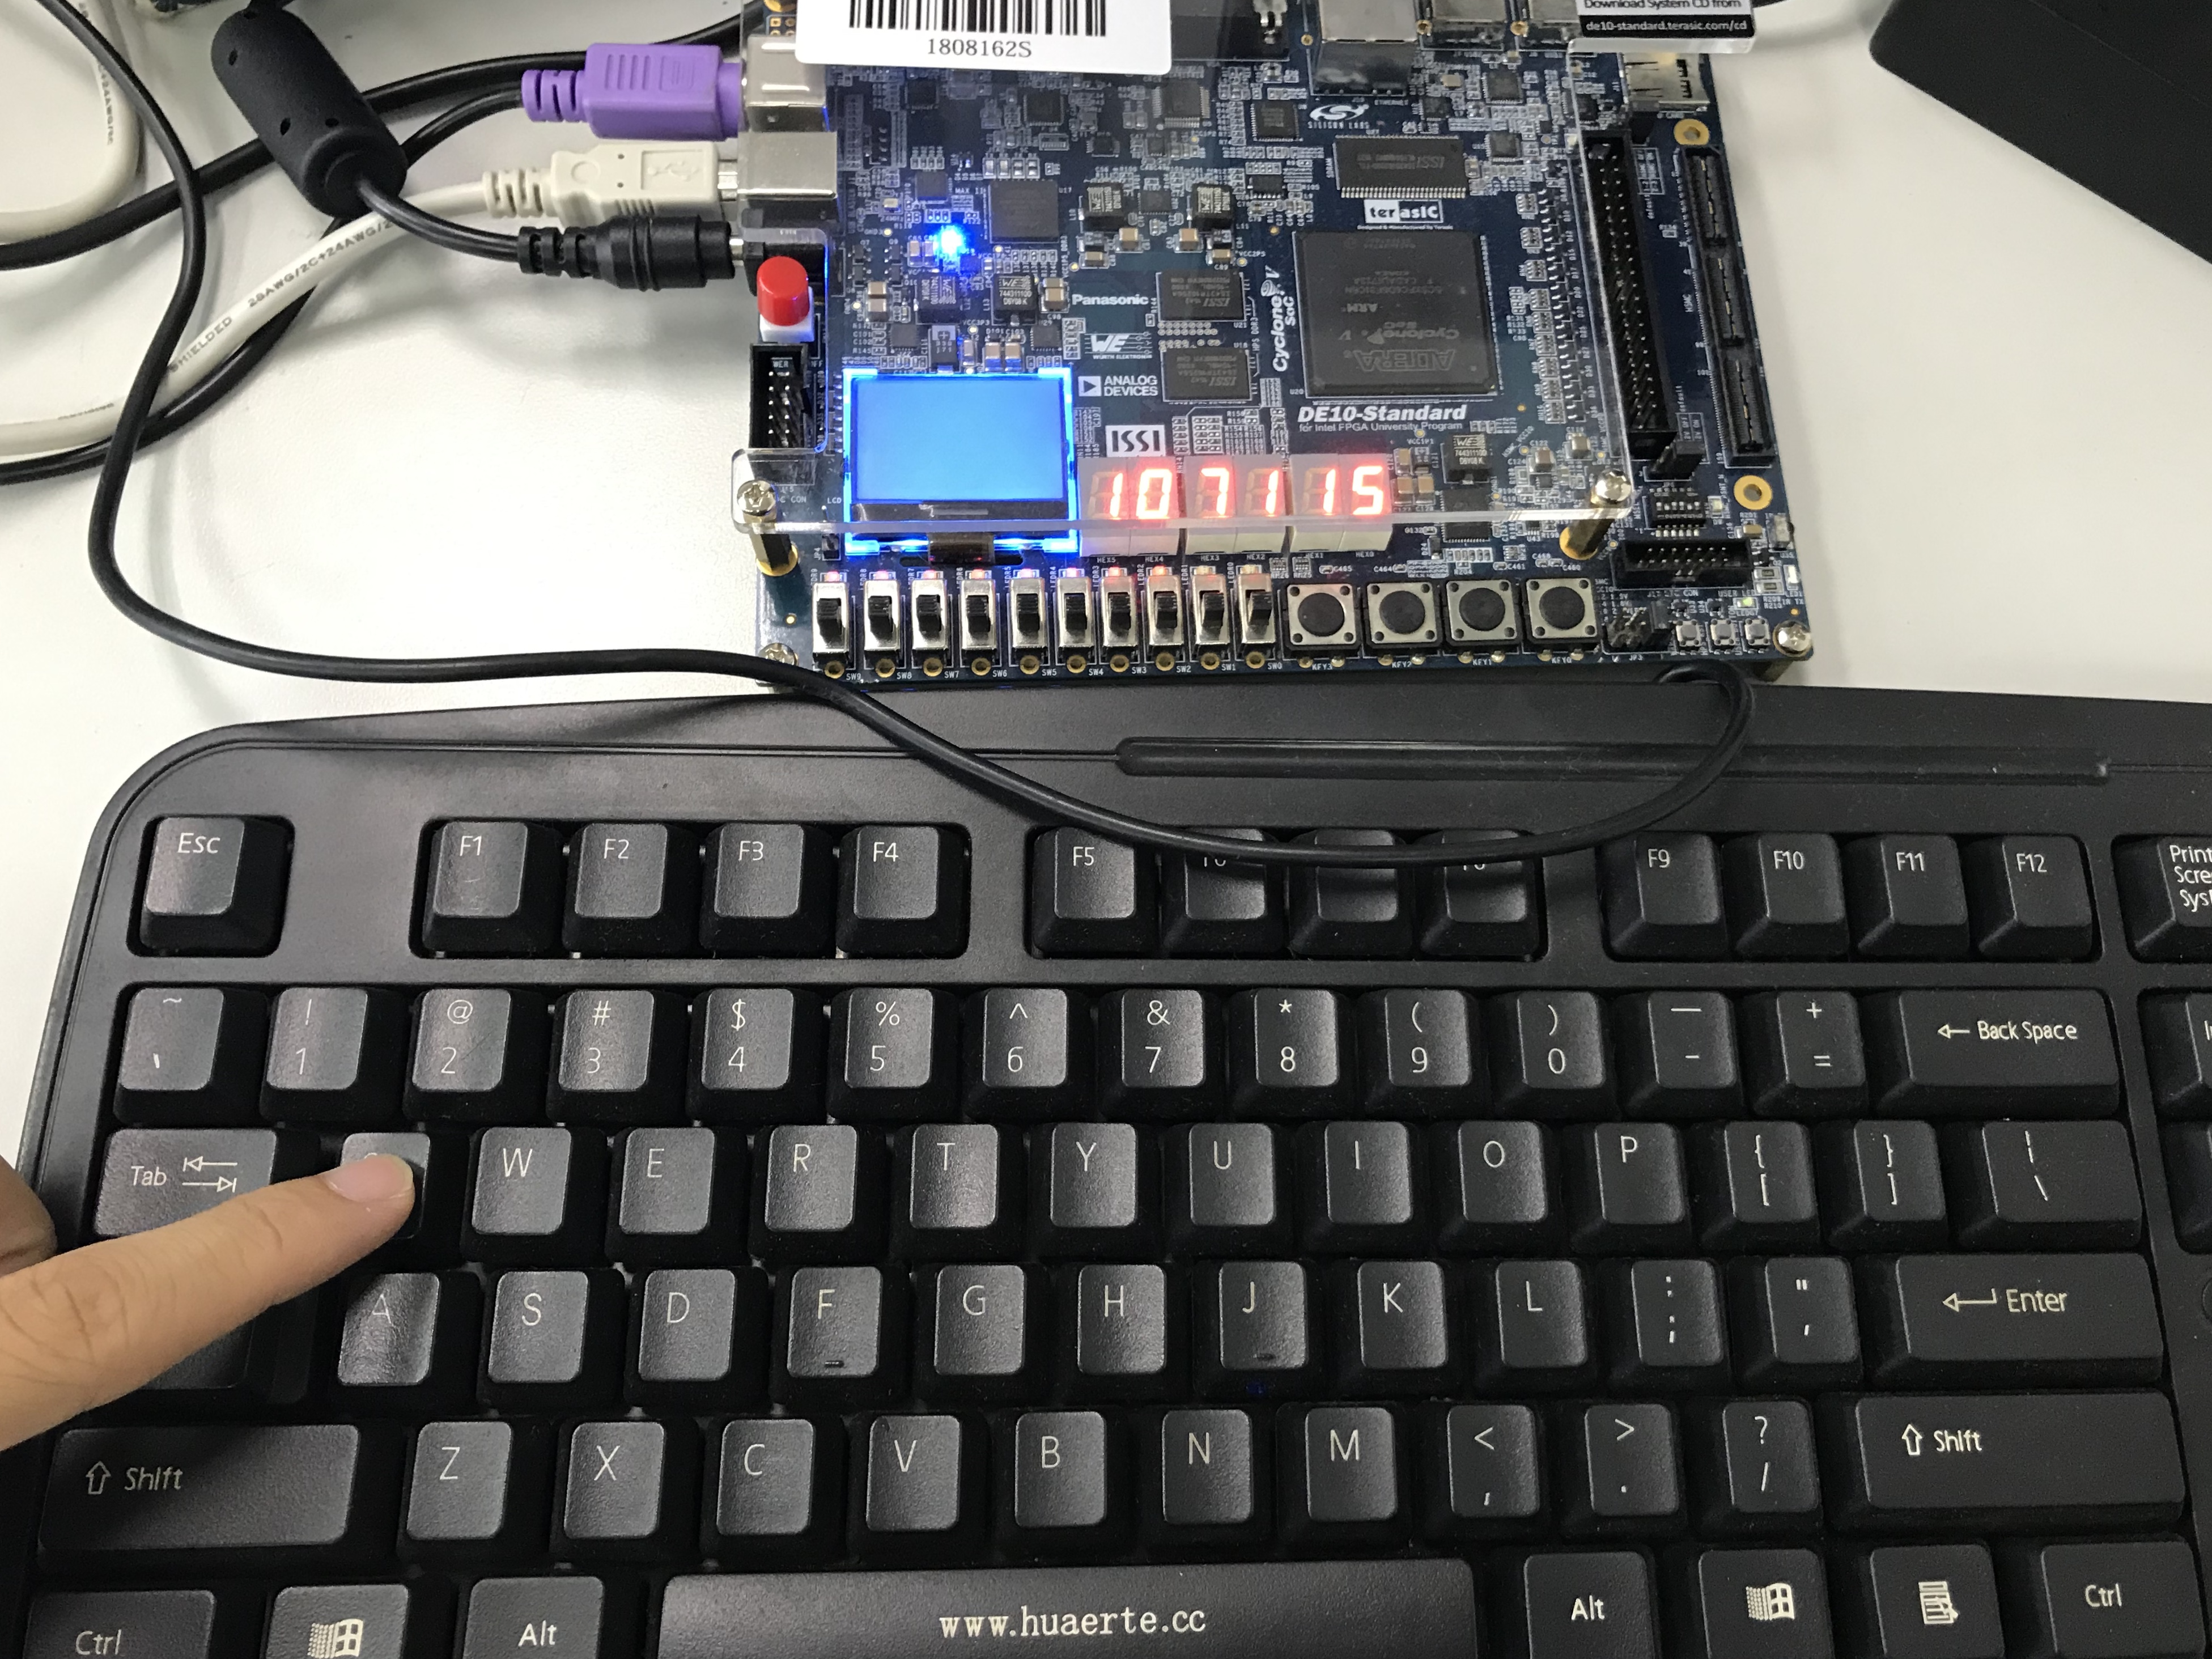
\includegraphics[width=0.45\textwidth]{fpga_normal.JPG}
  }
  \caption{普通按键}
  \label{fpga_normal}
\end{figure}

\begin{figure}[H]
  \centering
  \subfigure[FPGA Shift]{
    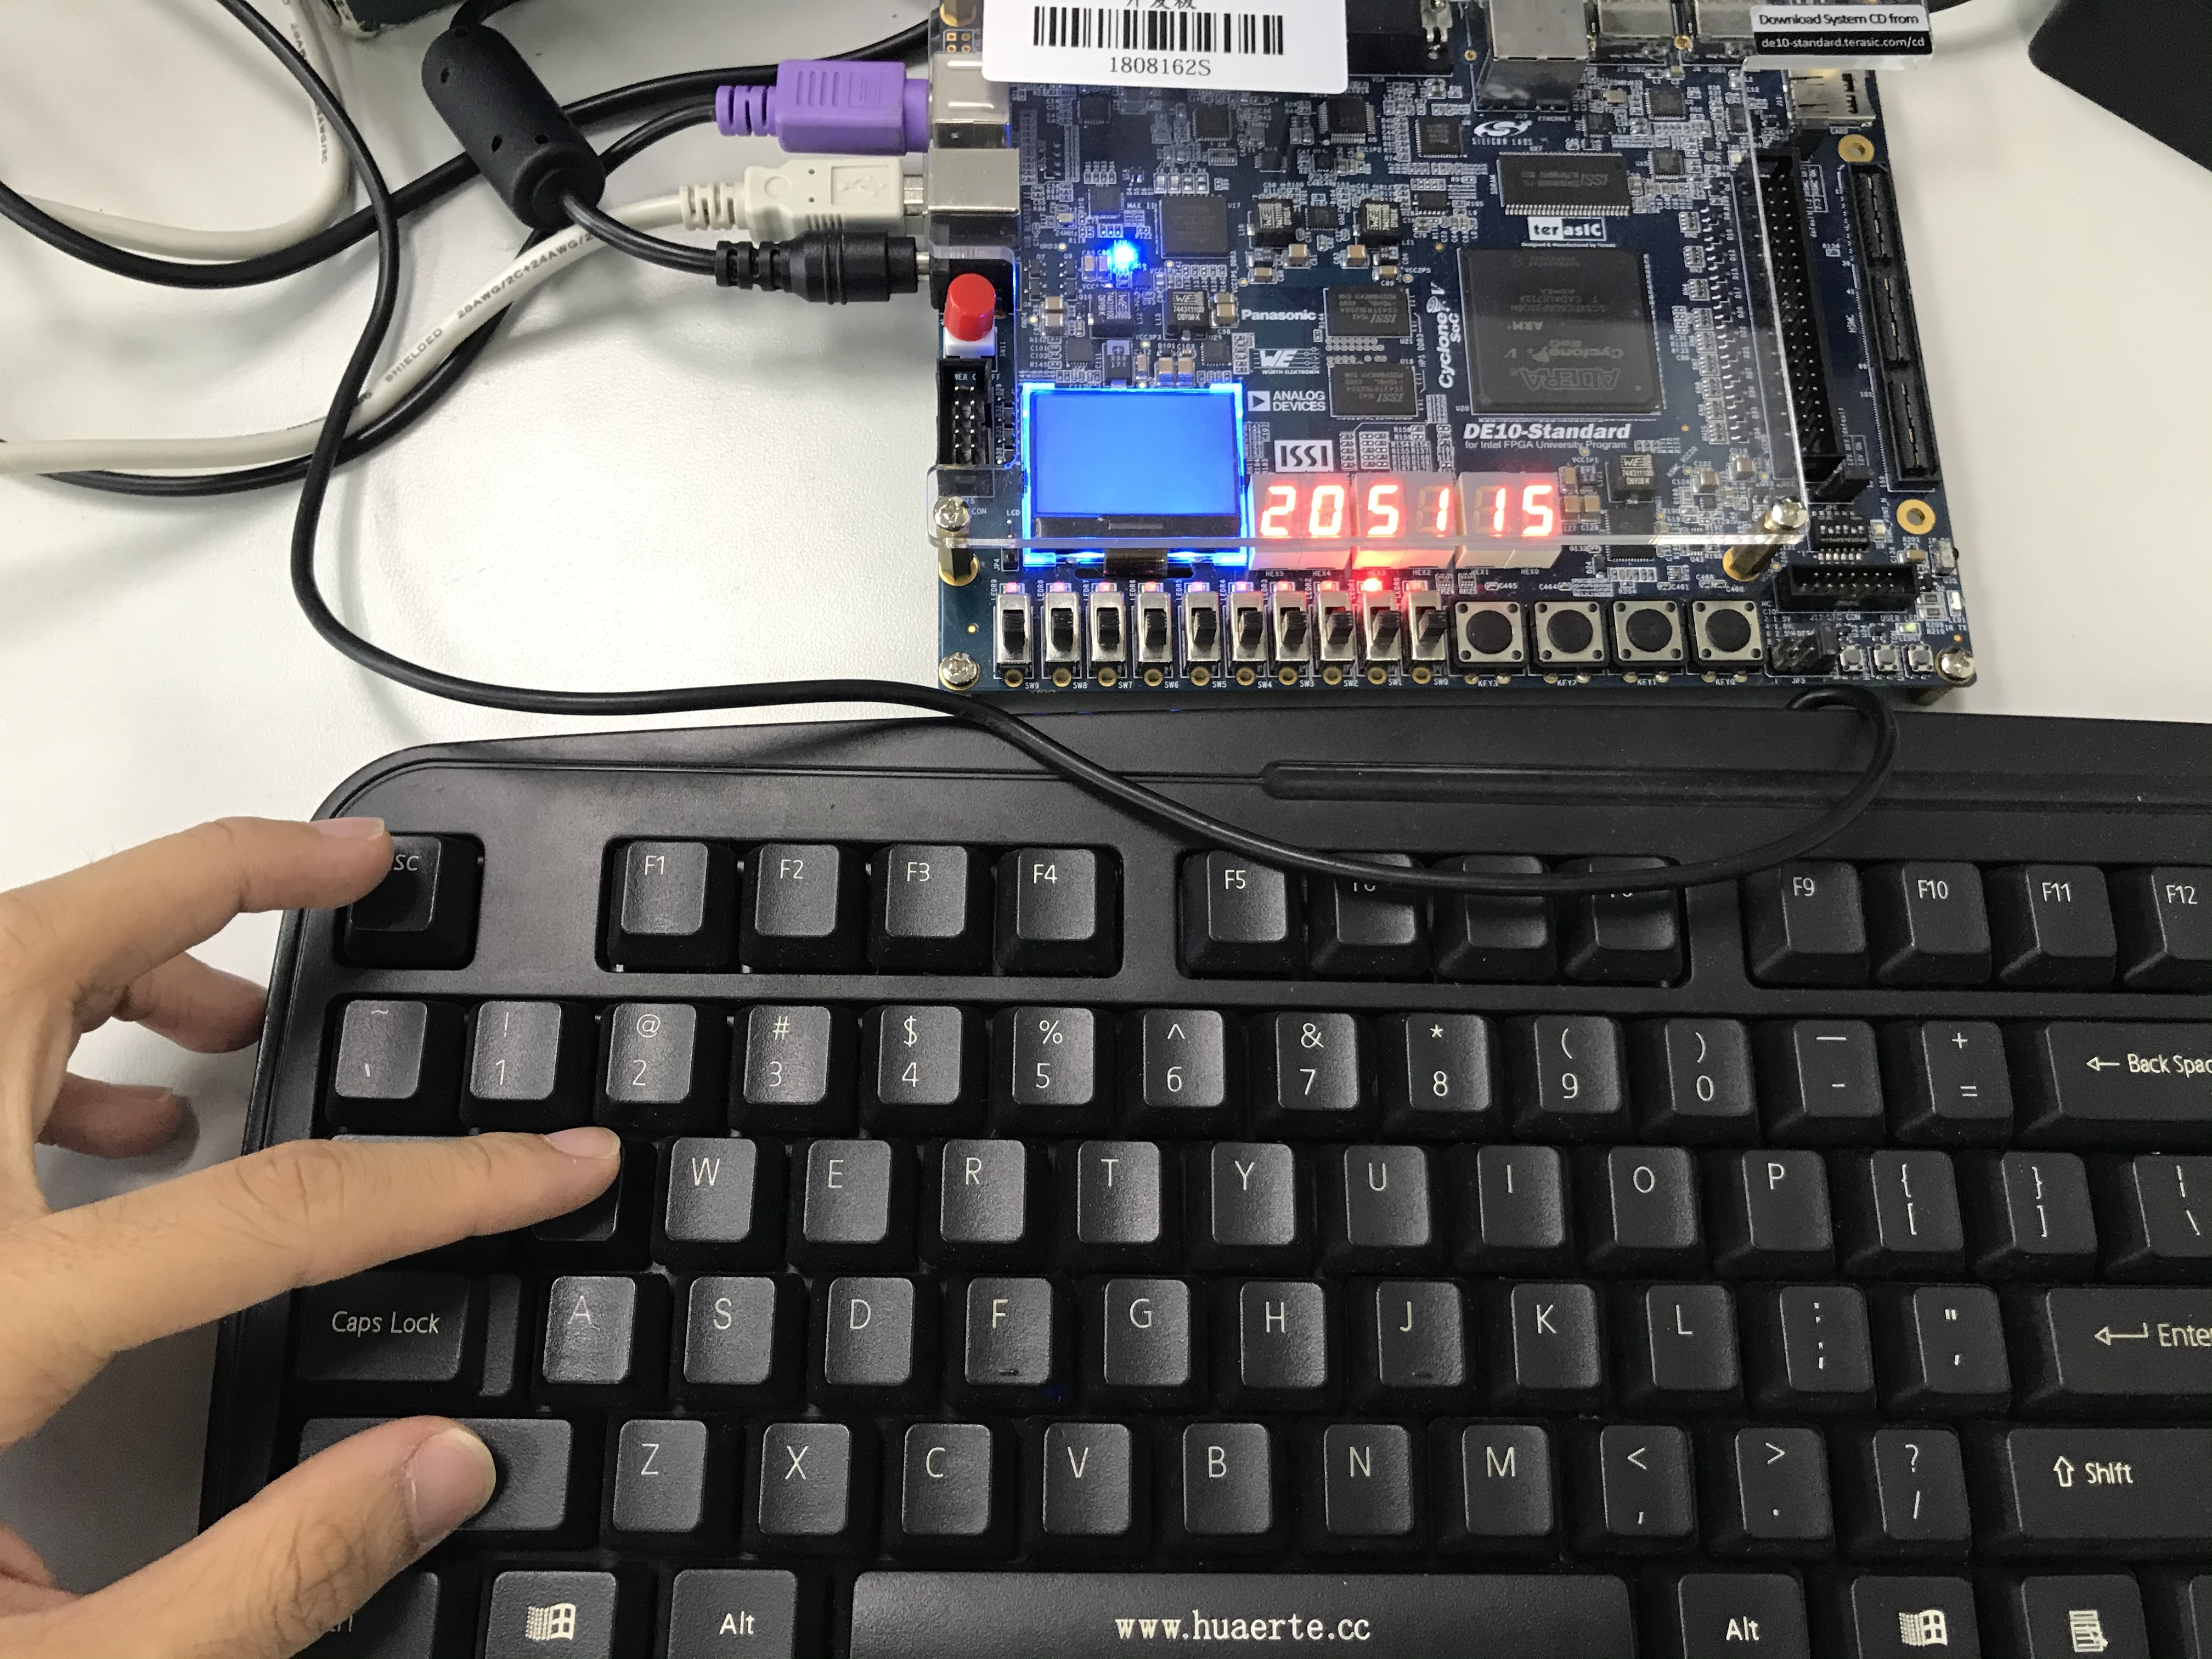
\includegraphics[width=0.3\textwidth]{fpga_shift.JPG}
  }
  \subfigure[FPGA Caps]{
    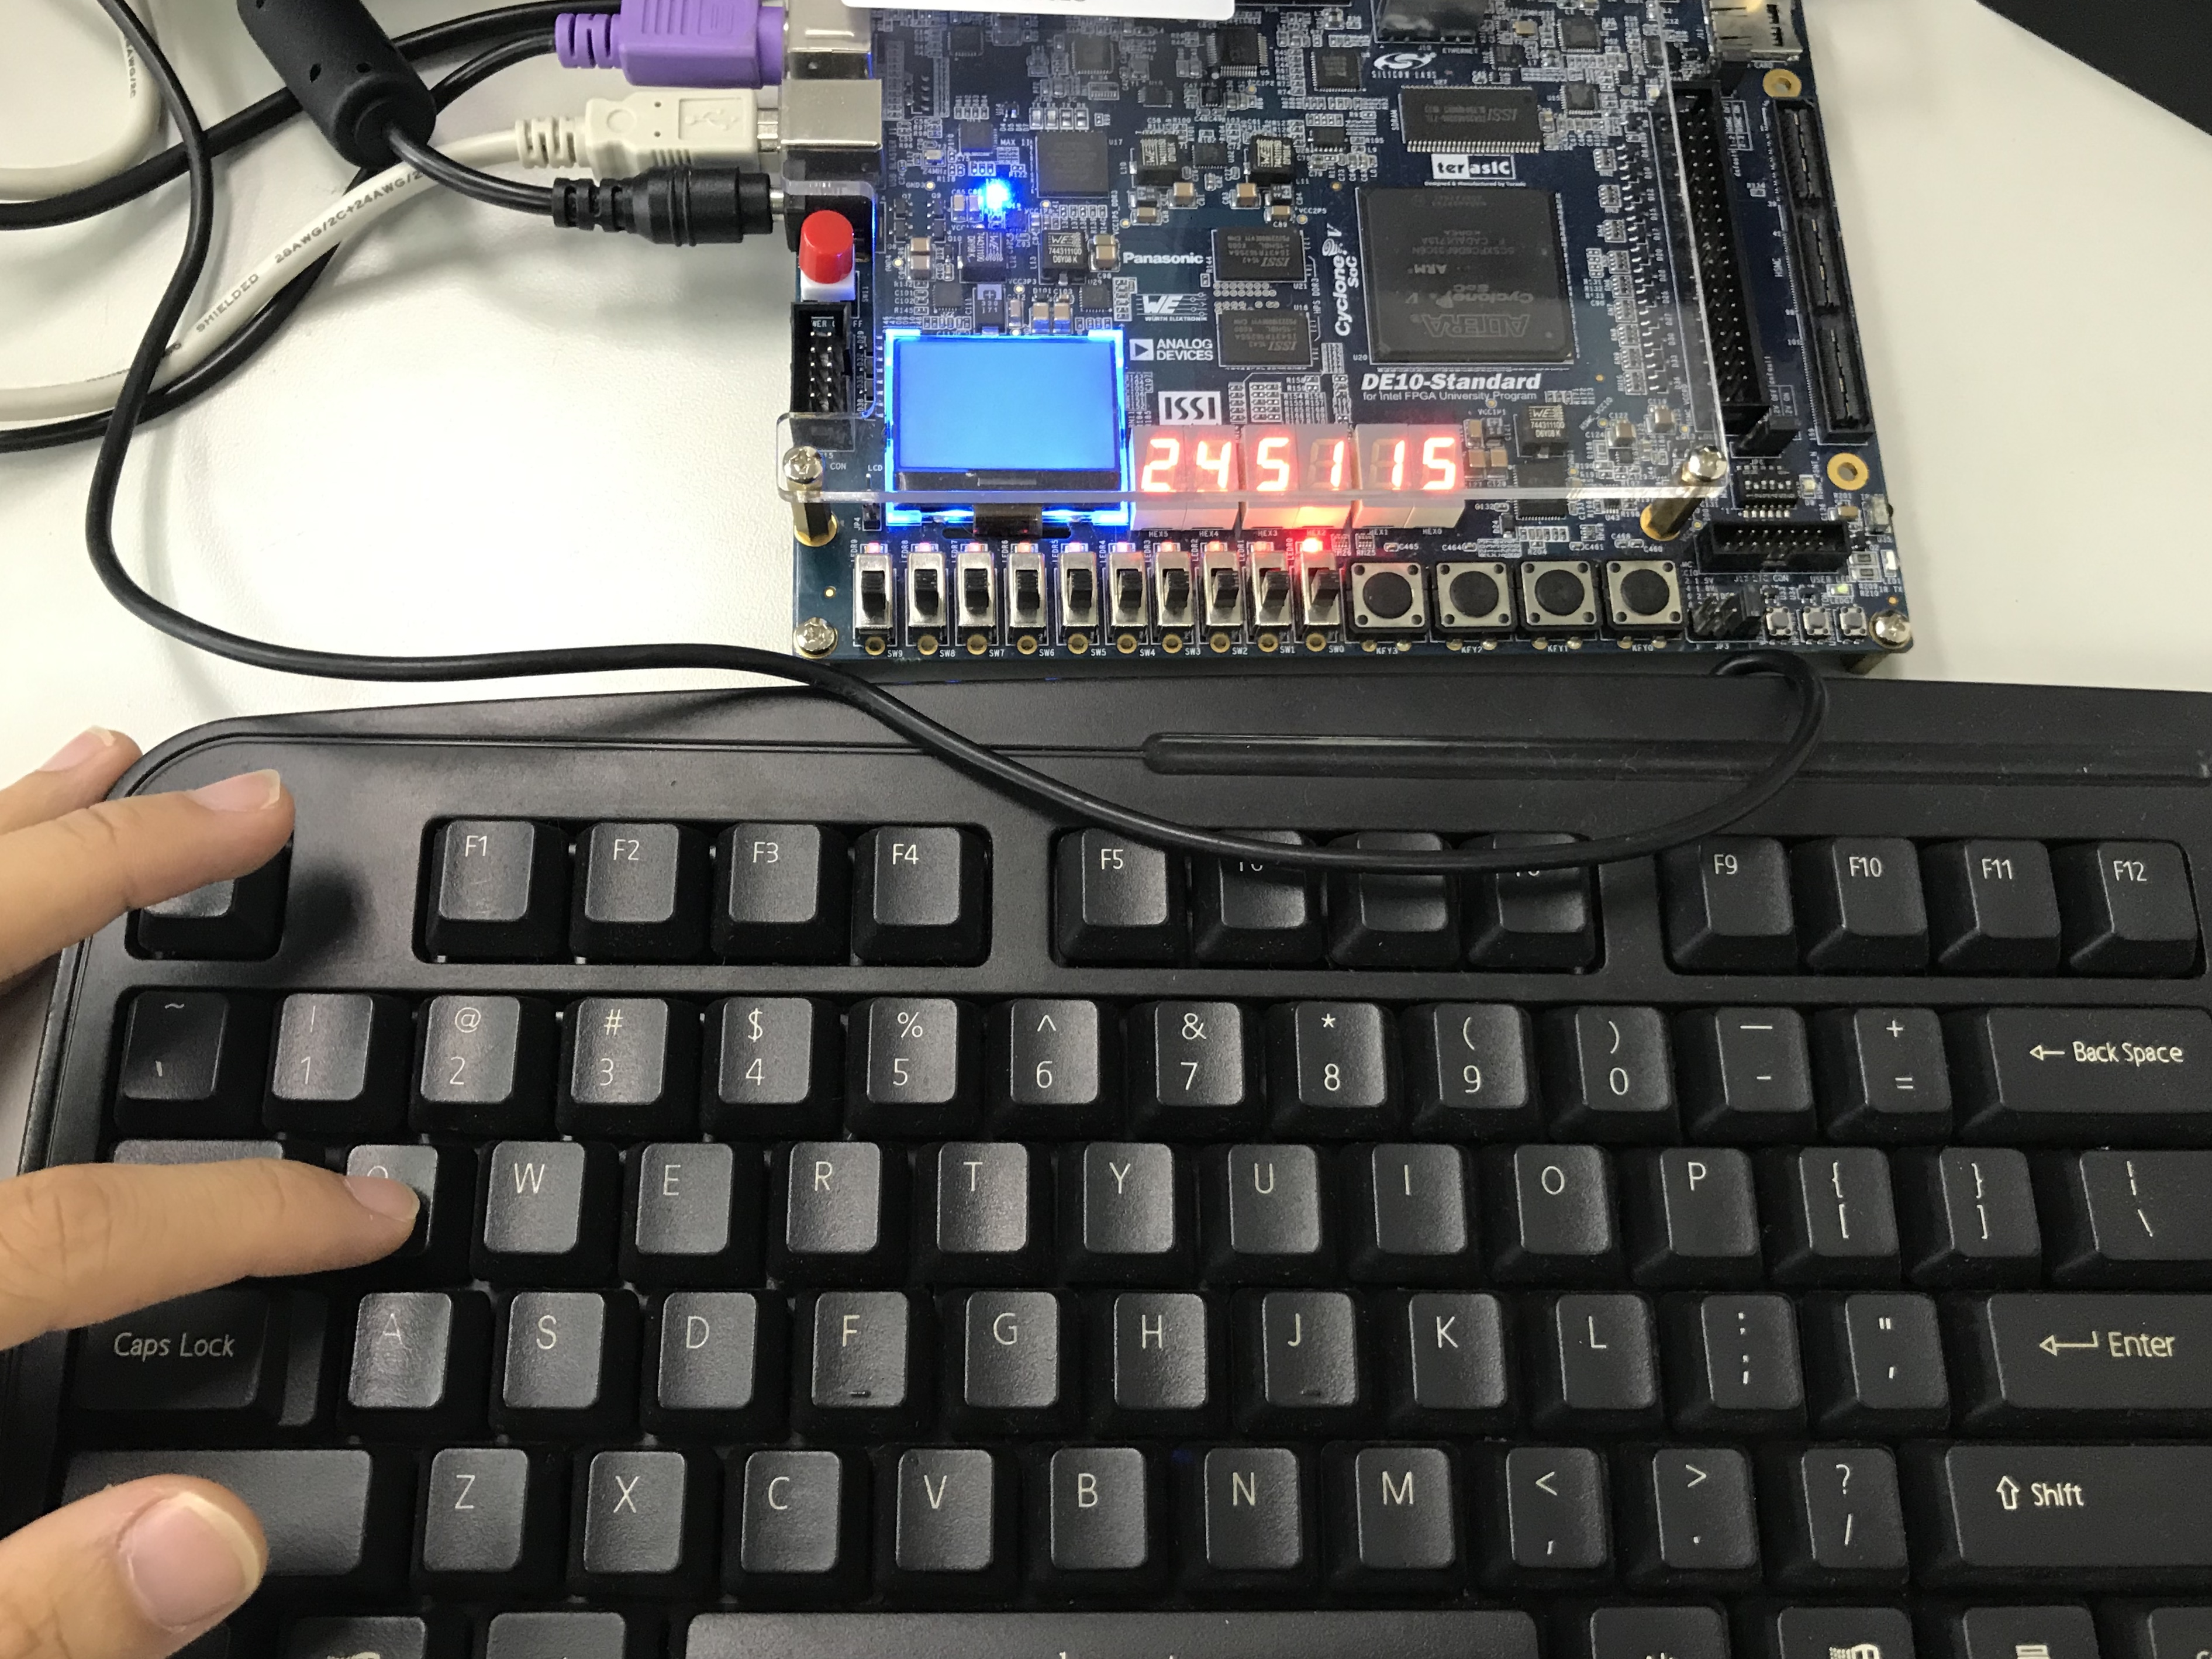
\includegraphics[width=0.3\textwidth]{fpga_caps.JPG}
  }
  \subfigure[FPGA CapsShift]{
    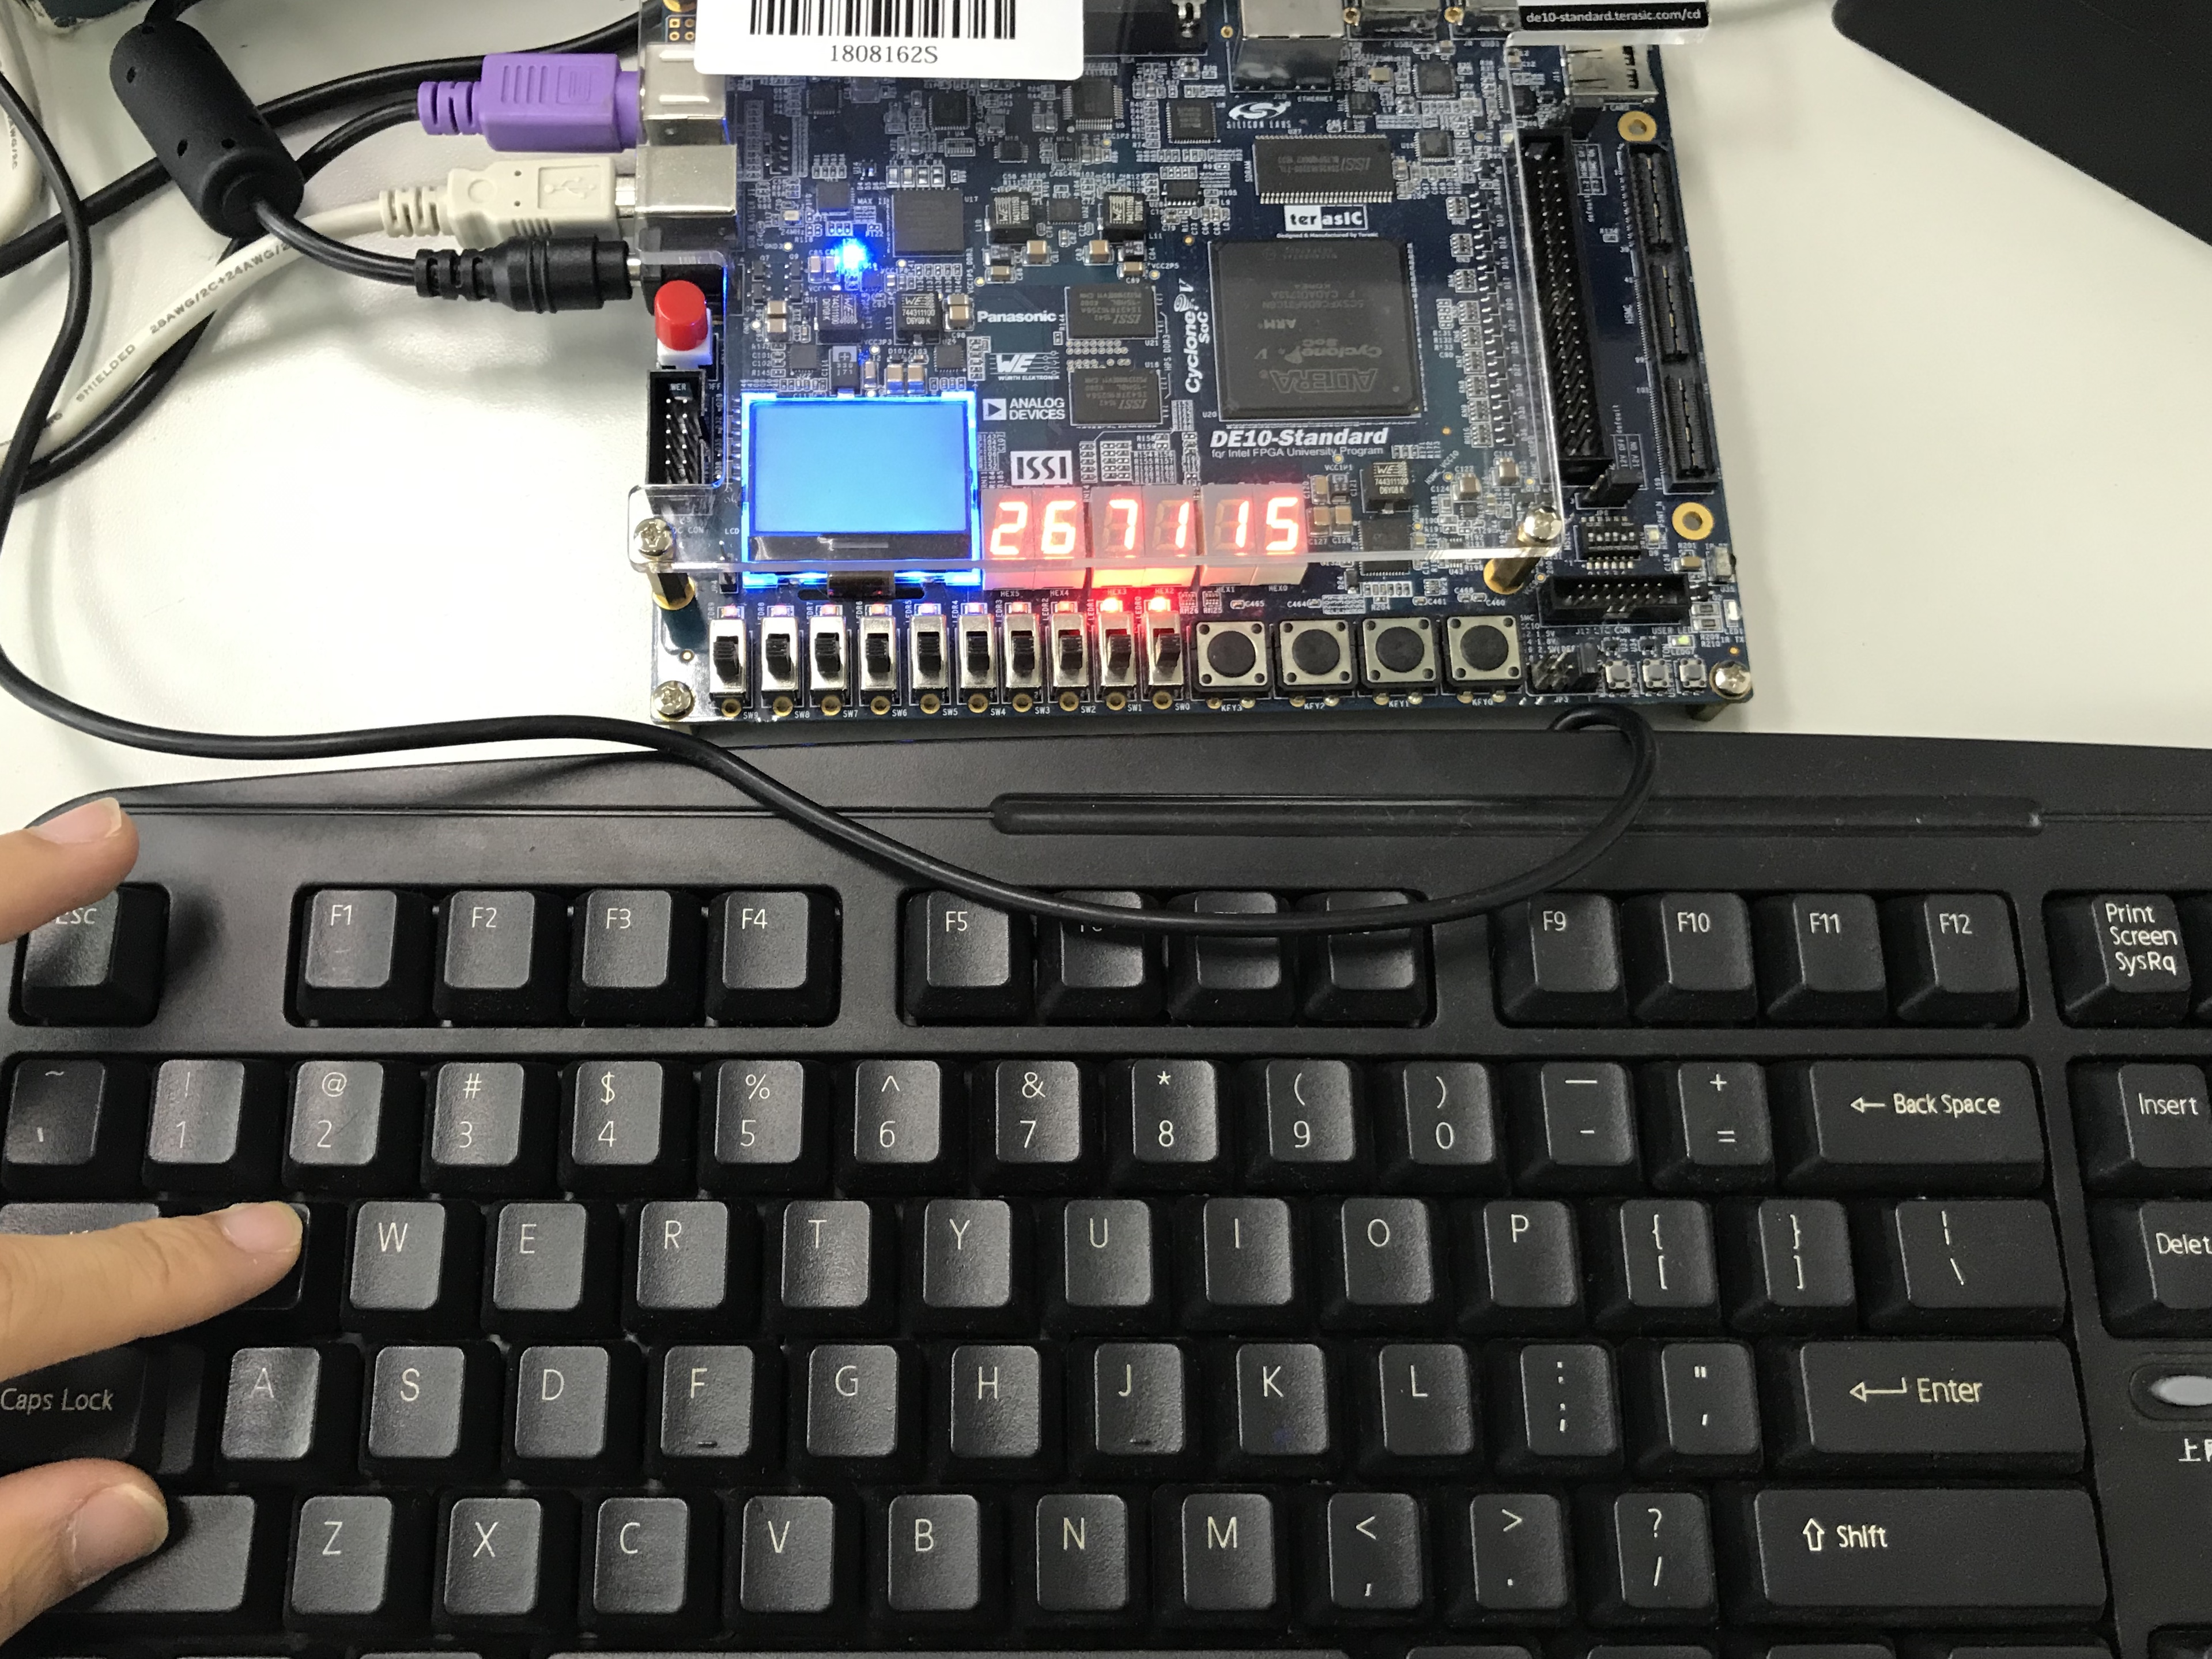
\includegraphics[width=0.3\textwidth]{fpga_capshift.JPG}
  }
  \caption{大写字符}
  \label{fpga_uppercase}
\end{figure}

\section{遇到的问题及解决办法}
\begin{itemize}
  \item 把一个模块设成顶层模块测试之后,忘记还原顶层模块
        就下载到FPGA上运行了……这bug我整整找了一下午……我太难了……
  \item 尽量通过绝对路径和txt文件初始化存储器,理由详见\ref*{bbsec:ascii}节
\end{itemize}

\section{得到的启示}
\begin{itemize}
  \item 找不到bug的时候多回忆回忆之前出过的bug,
        很多时候吃一堑并不能长一智,比如input参数的
        数据宽度我又双叒叕写错了……惨痛的教训不提了……
\end{itemize}

\section{意见和建议}
\begin{itemize}
  \item 实验8.2.4的代码8-4中,判断empty的if语句中
        为什么是``\mbox{r\_ptr+1'b1}''而不是
        ``\mbox{r\_ptr+3'b1}''\sout{(强迫症晚癌患者极度不适)}
\end{itemize}

\end{document}